The Method Multiplication approach involves decomposing the API into multiple interface methods,
with decomposition based on responsibility, functionality, parameter types, or the nullability of certain parameters.
This decomposition is a delicate balance between usability and API complexity; the functionality should not be overly
fine-grained or excessively spanned across multiple interface methods.

Figure~\ref{fig:mult_decomposition_by_type} illustrates the decomposition of the API based on IGMPv2 types.
The previous version of API (Figure~\ref{fig:sing_write_max_response_time}) is split into three interface methods,
each dedicated to a specific message type
\footnote{
    The subsequent diagrams exclude the calculation of the checksum, as it is irrelevant for illustrating API design.
    This omission remains consistent across every version of the example.
}.
This separation allows the removal of the \textit{igmpType} parameter from the interface method,
simplifying the input parameter checks in the implementation logic.

\begin{figure}[!htb]
    \centering
    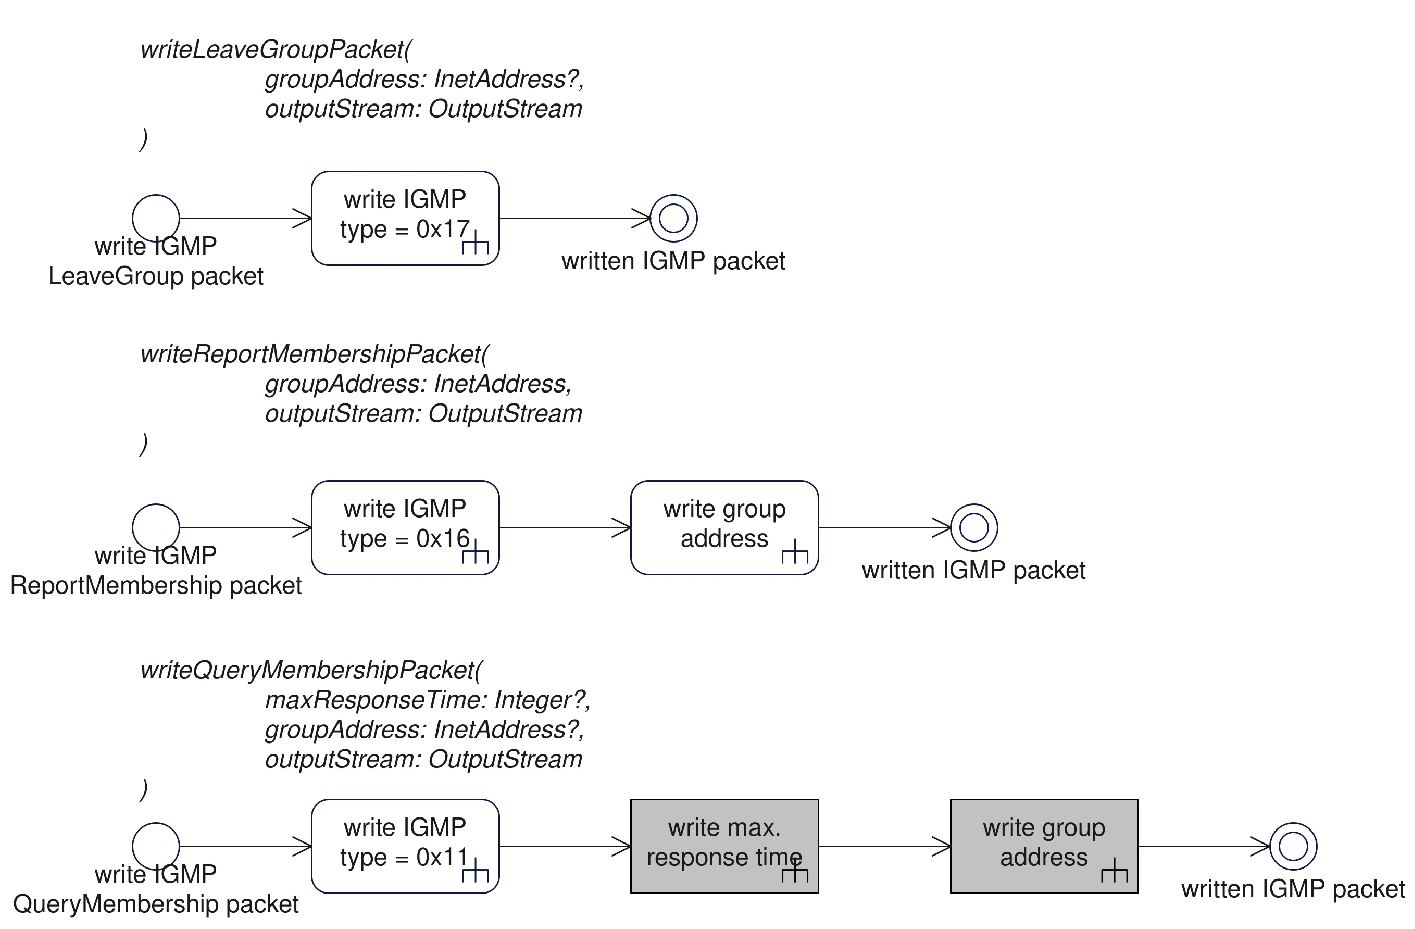
\includegraphics[width=1.0
    \textwidth]{mult_decomposition_by_type}
    \caption{Method Multiplication: Decomposition of API by type}
    \label{fig:mult_decomposition_by_type}
\end{figure}

In Figure~\ref{fig:mult_decomposition_by_type}, the writing of the IGMP Query Membership message remains complex due
to two optional parameters: \textit{maxResponseTime} and \textit{groupAddress}.
The \textit{groupAddress} is only \textit{0.0.0.0} in the case of the General Query message; otherwise,
it is a mandatory parameter.
To address this, it is sensible to split the interface method into two: one for the General Query message and another
for the Group-Specific Query message.
This decomposition is depicted in Figure~\ref{fig:mult_decomposition_by_function}.

\begin{figure}[!htb]
    \centering
    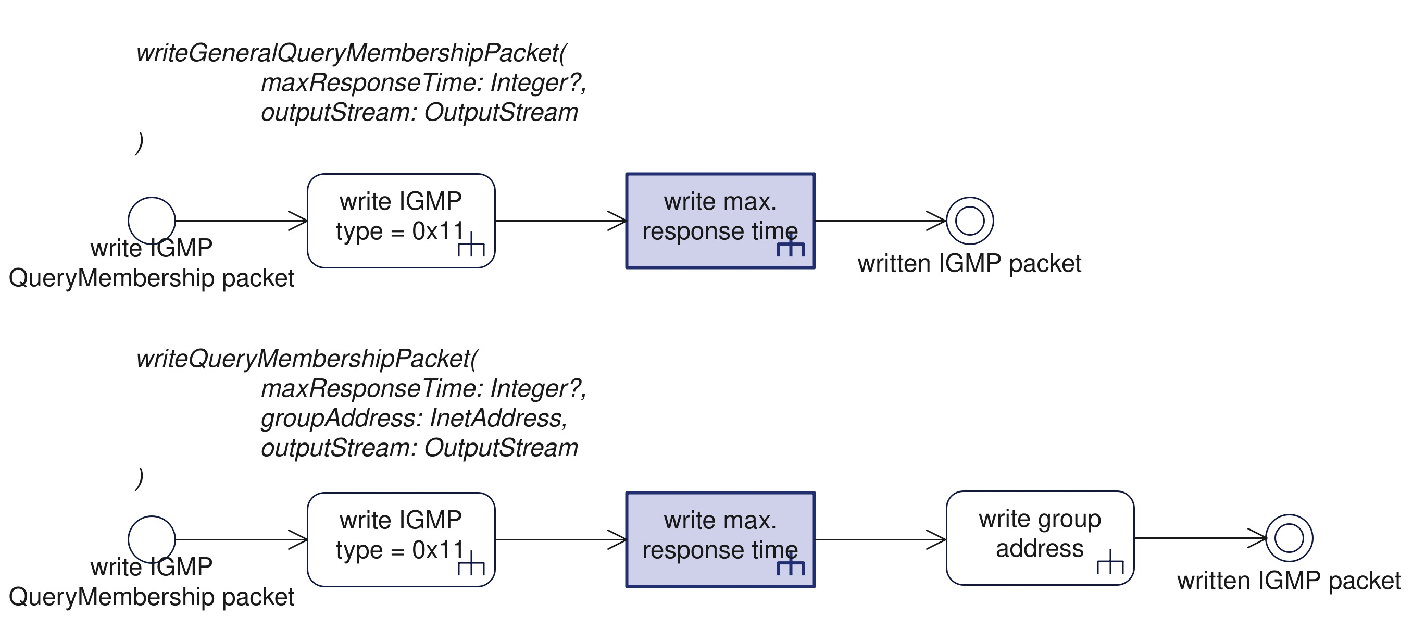
\includegraphics[width=1.0
    \textwidth]{mult_decomposition_by_function}
    \caption{Method Multiplication: Decomposition of API by functionality}
    \label{fig:mult_decomposition_by_function}
\end{figure}

Finally, Figure~\ref{fig:mult_decomposition_by_default_values} illustrates the split of the method for writing
the QueryMembership message into two overloaded interface methods - one with the \textit{maxResponseTime} parameter
and another without it, which internally sets a default value.
It is important to note that method overloading is not universally possible in all programming languages.
Moreover, it should be avoided if the methods have different functionalities.
In such cases, using different identifiers for the methods enhances readability.

\begin{figure}[!htb]
    \centering
    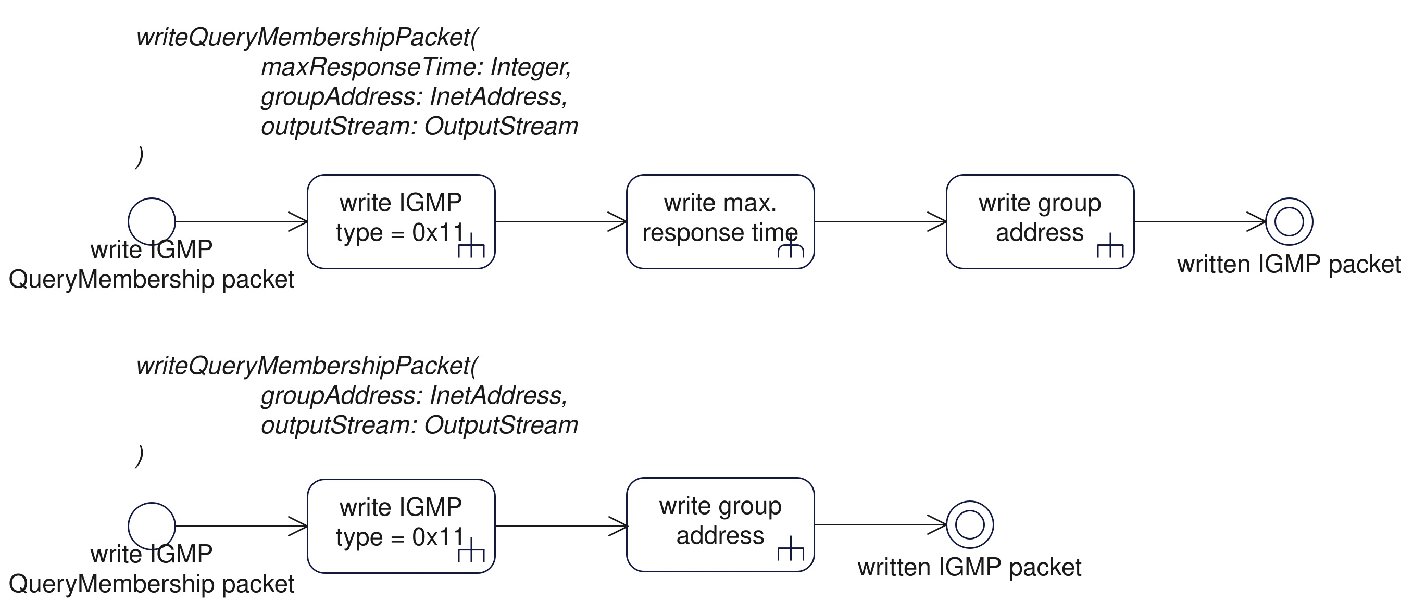
\includegraphics[width=1.0
    \textwidth]{mult_decomposition_by_default_values}
    \caption{Method Multiplication: Decomposition of API by default values}
    \label{fig:mult_decomposition_by_default_values}
\end{figure}

Other strategies for decomposition of methods include Replace Parameter with Explicit Methods or
Separate Query from Modifier refactoring patterns.
They are described in detail in the Refactoring: Improving the Design of Existing Code
book~\cite[Chapter~10]{fowler1999refactoring}.

Benefits of the Method Multiplication:

\begin{itemize}
    \item Enhanced readability and understandability:
    The API becomes more readable and understandable compared to the Singleton Interface Method.
    Well-chosen identifiers for interface methods make it easy to comprehend the purpose of the API method,
    often rendering the code self-documented.
    \item Improved maintainability:
    API maintainability is enhanced as updating or adding new functionality becomes easier.
    Changes are localized to the single interface method, simplifying the overall maintenance process.
    \item Enhanced robustness:
    The API becomes more robust as it prevents the invocation of methods with invalid parameter combinations.
    \item Mitigation of God Methods:
    The implementation of the API is distributed across multiple methods, addressing the issue of God Methods.
\end{itemize}

Drawbacks of the Method Multiplication:

\begin{itemize}
    \item Potential for God Classes:
    While the API is decomposed, there may still be a single service implemented by a class, leading to potential
    growth over time.
    Consideration of further division into multiple services, especially through Vertical Slicing, may be beneficial.
    \item Client decision overhead:
    Clients must decide which method to call, often necessitating the implementation and maintenance of another
    Facade layer on top of the API to hide the complexity around correct interface method calls.
    Read more about the Facade design pattern in the book Pattern-Oriented Software Architecture, Volume 4:
    A Pattern Language for Distributed Computing ~\cite[Chapter~12]{posa4}.
    \item Risk of Spaghetti Code in God Classes:
    The presence of God Classes may lead to Spaghetti Code, characterized by a lack of structure and organization.
    This can result from rushed or unplanned coding, leading to a complex and tangled control structure.
    Figure~\ref{fig:mult_spaghetti_code} shows an example of the Spaghetti Code in the early stage.
    There are multiple shared procedures that are called by API methods with unclear control flow.
    Internal functions tend to contain a lot of parameters that are passed between them.
    \footnote{
        The term Spaghetti Code is often attributed to computer scientist Edsger Dijkstra.
        He used it in his 1972 Turing Award lecture titled The Humble Programmer~\cite{dijkstra1972humble}.
    }
    \item API Rooting:
    Implementations of interface methods might simply call another common method, potentially internal or represented
    by another public interface method
    This implies that while the API is decomposed, the internal implementation remains
    in the Singleton Interface Method.
    Figure~\ref{fig:mult_api_rooting} provides an example of API Rooting.
\end{itemize}

\begin{figure}[!htb]
    \centering
    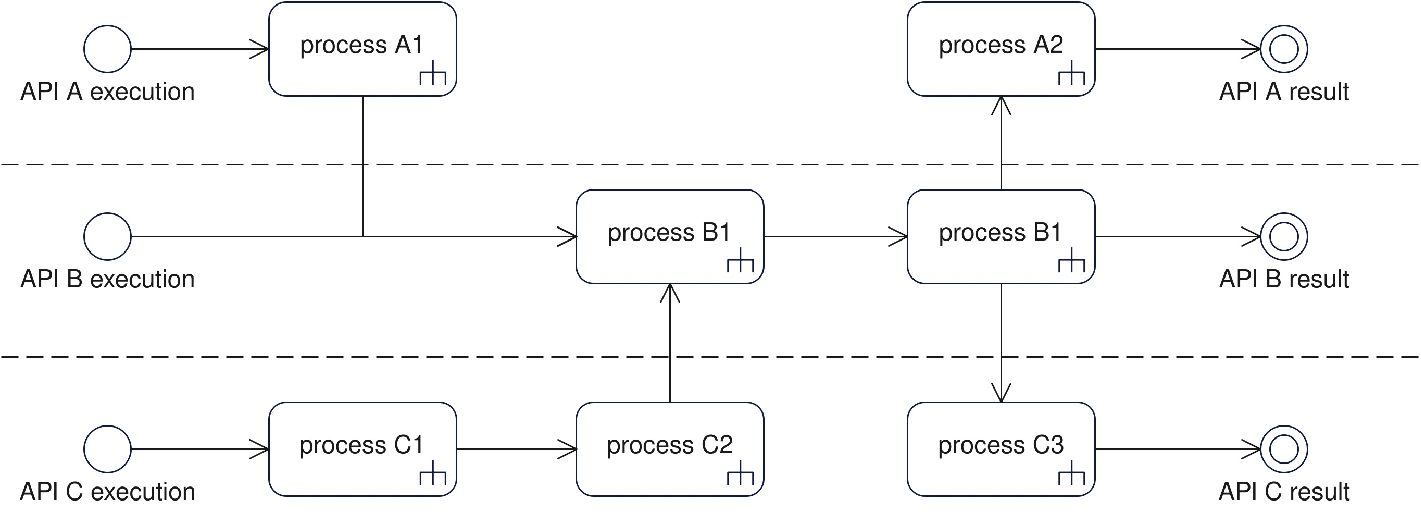
\includegraphics[width=1.0
    \textwidth]{mult_spaghetti_code}
    \caption{Method Multiplication: Germ of the Spaghetti Code}
    \label{fig:mult_spaghetti_code}
\end{figure}

\begin{figure}[!htb]
    \centering
    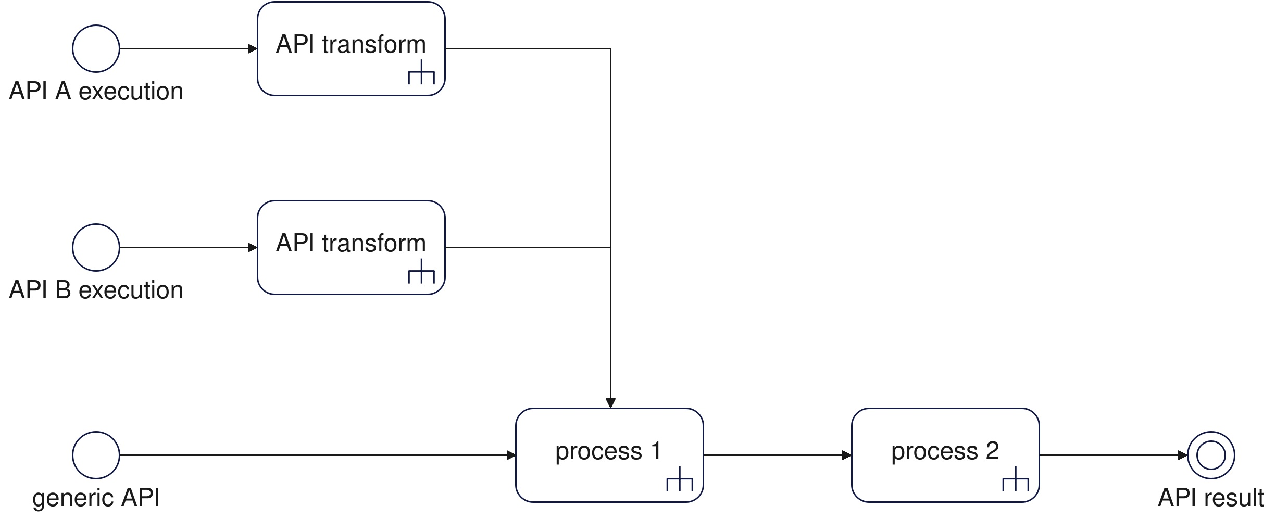
\includegraphics[width=1.0
    \textwidth]{mult_api_rooting}
    \caption{Method Multiplication: API Rooting}
    \label{fig:mult_api_rooting}
\end{figure}

Common use-cases of the Method Multiplication:

\begin{itemize}
    \item Decomposition by functionality:
    Decomposing the API by functionality into multiple interface methods is a common use-case for Method Multiplication.
    \item Overloading for parameter types:
    Overloading interface methods is utilized to support different types of input parameters.
\end{itemize}
